\documentclass[11pt,a4paper]{report} 
\usepackage[utf8]{inputenc}%encodage
\usepackage[T1]{fontenc}%accens
\usepackage[french]{babel}%français
%\usepackage{arev}%police
\usepackage[top=2cm,bottom=2cm,left=2cm,right=2cm]{geometry}
\frenchbsetup{StandardLists=true}
\usepackage{multicol}
\usepackage{shapepar}
\usepackage{nccrules}
\usepackage{ulem}
\usepackage{appendix}
\usepackage[squaren]{SIunits}
\usepackage{shorttoc}
\usepackage{eurosym}
\usepackage{color}
\usepackage{graphicx}
\usepackage{float}
\usepackage{wrapfig}
\usepackage{caption}
\usepackage{amsmath}
\usepackage{amssymb}
\usepackage{subfigure}
\setlength{\columnsep}{0cm}
\setlength{\parindent}{0pt}
\setlength{\columnseprule}{0pt}
\usepackage{fancyhdr}
\pagestyle{fancy}
\usepackage{array}
\usepackage{pgfgantt}
\usepackage{enumitem}
\usepackage{geometry}
\usepackage{multirow}
\usepackage{vmargin}

\parindent=0cm
\pagestyle{plain}
\usepackage{hyperref}

\begin{document}

\begin{titlepage}

\newcommand{\HRule}{\rule{\linewidth}{0.5mm}} % Defines a new command for the horizontal lines, change thickness here

\center % Center everything on the page
 
%----------------------------------------------------------------------------------------
%	HEADING SECTIONS
%----------------------------------------------------------------------------------------

\textsc{\LARGE ESAIP école d'ingénieur}\\[1.5cm] % Name of your university/college

\includegraphics[scale=0.5]{logo_esaip}\\[1cm] % Include a department/university logo - this will require the graphicx package
\textsc{\Large Dossier de conception}\\[0.5cm] % Major heading such as course name
\textsc{\large Projet Applicatif}\\[0.5cm] % Minor heading such as course title

%----------------------------------------------------------------------------------------
%	TITLE SECTION
%----------------------------------------------------------------------------------------

\HRule \\[0.4cm]
{ \huge \bfseries Annuaire ESAIP}\\[0.4cm] % Title of your document
\HRule \\[1.5cm]
 
%----------------------------------------------------------------------------------------
%	AUTHOR SECTION
%----------------------------------------------------------------------------------------

\begin{minipage}{0.4\textwidth}
\begin{flushleft} \large
\emph{\textbf {Author:}}\\
Baptiste \textsc{DEVES}\\ % Your name
Jordan \textsc{FRAUD-GELDOF}\\
Nicolas \textsc{GAUME}\\
Alexandre \textsc{JOURDOIS}\\
Nicolas \textsc{PIRON}\\
\end{flushleft}

\end{minipage}\\[2cm]

% If you don't want a supervisor, uncomment the two lines below and remove the section above
%\Large \emph{Author:}\\
%John \textsc{Smith}\\[3cm] % Your name

%----------------------------------------------------------------------------------------
%	DATE SECTION
%----------------------------------------------------------------------------------------

{\large \today}\\[2cm] % Date, change the \today to a set date if you want to be precise

\vfill % Fill the rest of the page with whitespace

\end{titlepage}
%renommer la table des matières en sommaire
\renewcommand{\contentsname}{Sommaire} 
%table des matières (position)
\tableofcontents

%\part{Partie 1}
	\chapter{Rappels sur le projet}
		De notre temps les avancés technologiques sont infinies, à l'inverse des ressources de notre planète. C'est dans le but préserver notre environnement que le green IT à vu le jour dans les année 90. Divers manifestations dans ce domaine ont été créées pour sensibiliser les populations mais surtout les techniciens et ingénieurs de demain à la conception éco-responsable. Cette année le GreenIT a permis à différentes écoles de France et d'Europe de constituer des équipes de 5 personnes et de se rencontrer dans une compétition  où la récompense était offerte à ceux qui réaliserait l'application web la plus green et avec la meilleure expérience utilisateur. Le défis de cette année était de réaliser une application web d'annuaire de dentistes. Dans la continuité du Design4Green nous avons décidé de réaliser un annuaire adapté à l'ESAIP.
		\section{Diagramme de Gantt}
		\begin{center}
			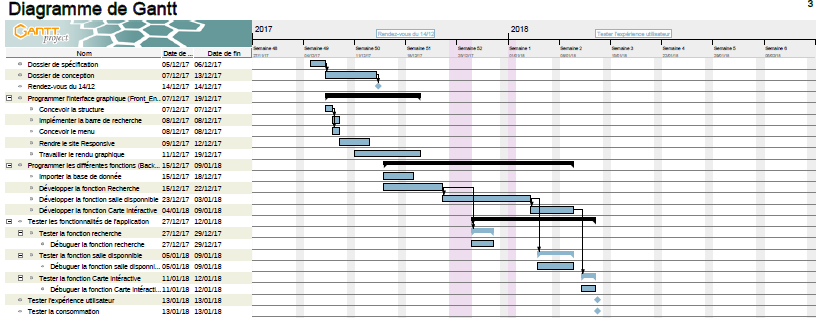
\includegraphics[angle=90,scale=1]{gantt}
		\end{center}
	\chapter{Fonctions détaillées}
		\section{Fonctions principales}
\emph{Fonction de recherche de personne :}\\

Cette fonction s'appuiera sur la base de données de l’esaip pour avoir accès aux noms et photos de toutes les personnes présentes à l’école.\\
\\
Cette recherche est nécessaire si l’on désire connaitre un membre d’une association, une personne du département relations internationales ou autre.\\
\\
Cette fonction permettra de rechercher une personne en fonction de son domaine de compétence et retournera ainsi l’emplacement de son bureau, sa photo et sa fonction au sein de l’école.\\
\\
\emph{Fonction de recherche service de l’école :}\\
\\Cette fonctionnalité a émergé suite à notre entrée à l’esaip. En effet quand nous sommes arrivés nous étions perdus et ne savions absolument pas où se trouvaient les différents services de l’école. Cette fonction permettra à n’importe quel nouvel arrivant de saisir le nom d’un service de l’établissement et ainsi se renseigner sur sa localisation.\\

Cette fonctionnalité fournira à l’utilisateur un plan de l’école et le nom du bâtiment dans lequel se trouve le service. Nous ajouterons également le nom des différentes personnes qui gèrent ce service.\\

\emph{Fonction d'affichage des données :}  \\
\\
Chaque personnes ou salles sélectionnés possèdent des données qui lui sont propres. C'est données devront pouvoir être affichées sont une page web spécifique.\\
\\
\\
\\
	\section{Fonctions secondaires} 
\emph{Fonction de recherche de salle :}  \\
\\Cette idée nous est venue alors que nous cherchions une salle informatique pour travailler un projet. En effet nous avons passé 20 min à errer dans l’esaip à la recherche d’une salle de libre, le co-working étant plein. 
A terme, cette fonction permettra à l’utilisateur de faire une recherche par critère (salle info ou non) et ainsi savoir quelle salle est actuellement disponible.
\\
\\Cette fonctionnalité renverra le numéro de(s) salle(s) disponible(s) ainsi que des renseignements sur cette dernière : son emplacement, PC ou non, bâtiment.\\
\\
\emph{Fonction afficher salle libre :}	\\
\\Nous aimerions pouvoir afficher les salles libres en temps réelle afin de permettre aux personnes souhaitant travailler de pouvoir être informer rapidement.		
	\chapter{Diagrammes UML}
		\section{Diagrammes des cas d'utilisations}
			\begin{center}
					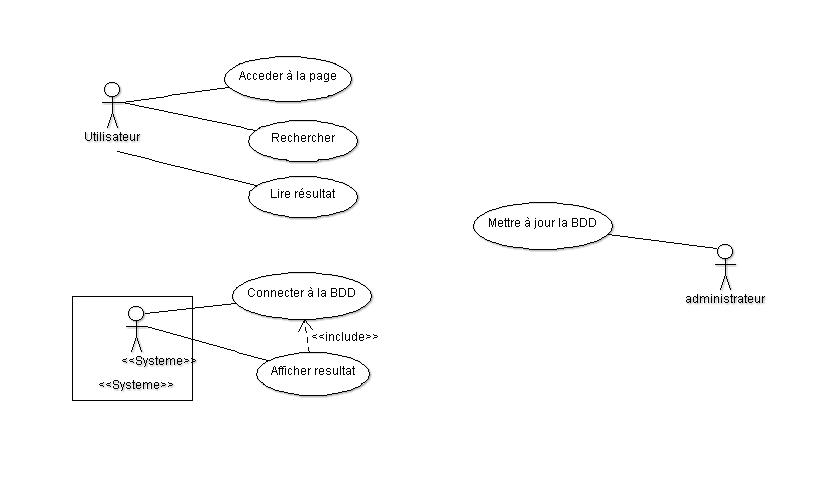
\includegraphics[scale=0.6]{d3}
			\end{center}
			
		\section{Diagrammes des classes}
				\begin{center}
					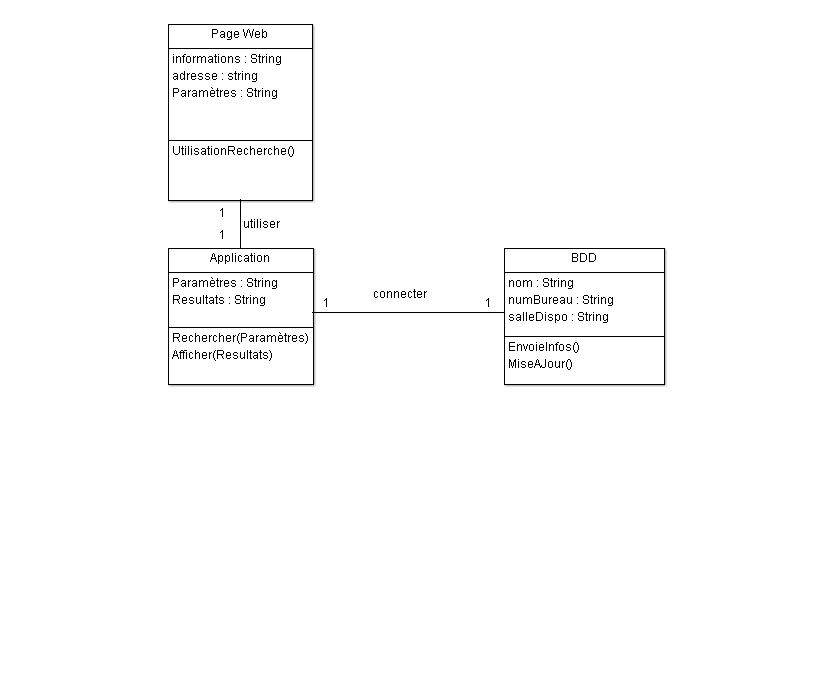
\includegraphics[scale=0.6]{classes}
				\end{center}
		\section{Diagrammes de séquences}
		\begin{center}
			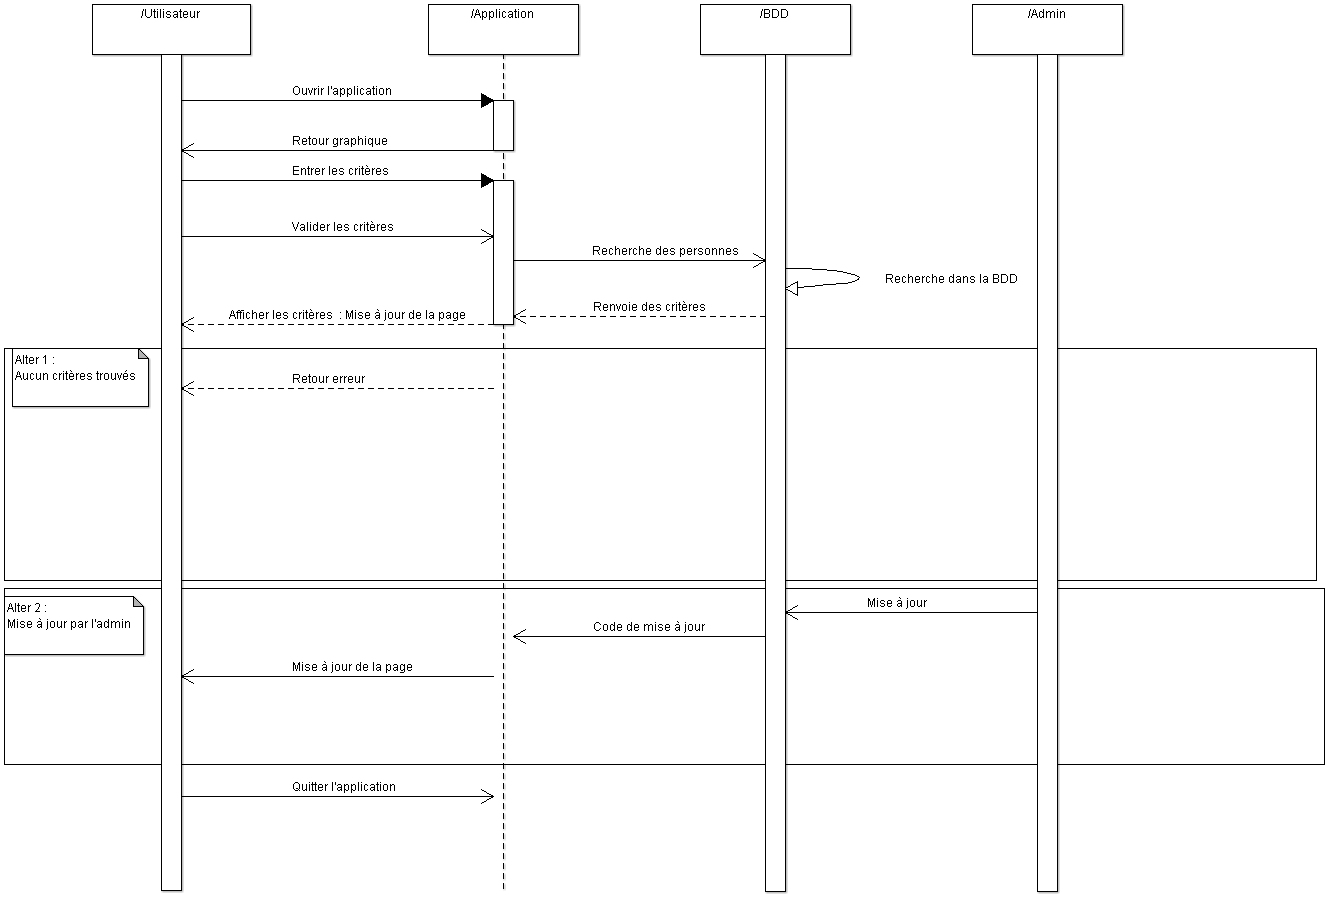
\includegraphics[angle=90,scale=0.45]{sequences}
		\end{center}
	\chapter{Interfaces HTML/CSS}
		\section{GreenIT}
			L'annuaire que nous proposons, sous forme de site web, est étudié pour être le plus green possible. Pour se faire le site devra respecter au mieux les 115 bonnes pratiques d'éco-conception web. Ces règles sont relatives aux différents langages de programmations utilisés :
	\begin{itemize}
			\item Conception
			\item  Templating
			\item Code CLient
			\item Code Serveur
			\item Hébergement
			\item Contenu
	\end{itemize}		
		\section{Expérience utilisateur}
		Un des points importants du Design4Green était l'expérience utilisateur. Pour cela nous devons proposer à des utilisateurs de tester notre site. Nous choisirons des utilisateurs issus des différents types d'acteurs que nous avons identifiés. A savoir :
		\begin{itemize}
			\item les étudiants
			\item  le personnel administratif
			\item les enseignants
		\end{itemize}
\end{document}

